% Options for packages loaded elsewhere
\PassOptionsToPackage{unicode}{hyperref}
\PassOptionsToPackage{hyphens}{url}
%
\documentclass[
]{article}
\usepackage{lmodern}
\usepackage{amssymb,amsmath}
\usepackage{ifxetex,ifluatex}
\ifnum 0\ifxetex 1\fi\ifluatex 1\fi=0 % if pdftex
  \usepackage[T1]{fontenc}
  \usepackage[utf8]{inputenc}
  \usepackage{textcomp} % provide euro and other symbols
\else % if luatex or xetex
  \usepackage{unicode-math}
  \defaultfontfeatures{Scale=MatchLowercase}
  \defaultfontfeatures[\rmfamily]{Ligatures=TeX,Scale=1}
\fi
% Use upquote if available, for straight quotes in verbatim environments
\IfFileExists{upquote.sty}{\usepackage{upquote}}{}
\IfFileExists{microtype.sty}{% use microtype if available
  \usepackage[]{microtype}
  \UseMicrotypeSet[protrusion]{basicmath} % disable protrusion for tt fonts
}{}
\makeatletter
\@ifundefined{KOMAClassName}{% if non-KOMA class
  \IfFileExists{parskip.sty}{%
    \usepackage{parskip}
  }{% else
    \setlength{\parindent}{0pt}
    \setlength{\parskip}{6pt plus 2pt minus 1pt}}
}{% if KOMA class
  \KOMAoptions{parskip=half}}
\makeatother
\usepackage{xcolor}
\IfFileExists{xurl.sty}{\usepackage{xurl}}{} % add URL line breaks if available
\IfFileExists{bookmark.sty}{\usepackage{bookmark}}{\usepackage{hyperref}}
\hypersetup{
  pdftitle={emmeans Notes},
  pdfauthor={F.A. Barrios},
  hidelinks,
  pdfcreator={LaTeX via pandoc}}
\urlstyle{same} % disable monospaced font for URLs
\usepackage[margin=1in]{geometry}
\usepackage{color}
\usepackage{fancyvrb}
\newcommand{\VerbBar}{|}
\newcommand{\VERB}{\Verb[commandchars=\\\{\}]}
\DefineVerbatimEnvironment{Highlighting}{Verbatim}{commandchars=\\\{\}}
% Add ',fontsize=\small' for more characters per line
\usepackage{framed}
\definecolor{shadecolor}{RGB}{248,248,248}
\newenvironment{Shaded}{\begin{snugshade}}{\end{snugshade}}
\newcommand{\AlertTok}[1]{\textcolor[rgb]{0.94,0.16,0.16}{#1}}
\newcommand{\AnnotationTok}[1]{\textcolor[rgb]{0.56,0.35,0.01}{\textbf{\textit{#1}}}}
\newcommand{\AttributeTok}[1]{\textcolor[rgb]{0.77,0.63,0.00}{#1}}
\newcommand{\BaseNTok}[1]{\textcolor[rgb]{0.00,0.00,0.81}{#1}}
\newcommand{\BuiltInTok}[1]{#1}
\newcommand{\CharTok}[1]{\textcolor[rgb]{0.31,0.60,0.02}{#1}}
\newcommand{\CommentTok}[1]{\textcolor[rgb]{0.56,0.35,0.01}{\textit{#1}}}
\newcommand{\CommentVarTok}[1]{\textcolor[rgb]{0.56,0.35,0.01}{\textbf{\textit{#1}}}}
\newcommand{\ConstantTok}[1]{\textcolor[rgb]{0.00,0.00,0.00}{#1}}
\newcommand{\ControlFlowTok}[1]{\textcolor[rgb]{0.13,0.29,0.53}{\textbf{#1}}}
\newcommand{\DataTypeTok}[1]{\textcolor[rgb]{0.13,0.29,0.53}{#1}}
\newcommand{\DecValTok}[1]{\textcolor[rgb]{0.00,0.00,0.81}{#1}}
\newcommand{\DocumentationTok}[1]{\textcolor[rgb]{0.56,0.35,0.01}{\textbf{\textit{#1}}}}
\newcommand{\ErrorTok}[1]{\textcolor[rgb]{0.64,0.00,0.00}{\textbf{#1}}}
\newcommand{\ExtensionTok}[1]{#1}
\newcommand{\FloatTok}[1]{\textcolor[rgb]{0.00,0.00,0.81}{#1}}
\newcommand{\FunctionTok}[1]{\textcolor[rgb]{0.00,0.00,0.00}{#1}}
\newcommand{\ImportTok}[1]{#1}
\newcommand{\InformationTok}[1]{\textcolor[rgb]{0.56,0.35,0.01}{\textbf{\textit{#1}}}}
\newcommand{\KeywordTok}[1]{\textcolor[rgb]{0.13,0.29,0.53}{\textbf{#1}}}
\newcommand{\NormalTok}[1]{#1}
\newcommand{\OperatorTok}[1]{\textcolor[rgb]{0.81,0.36,0.00}{\textbf{#1}}}
\newcommand{\OtherTok}[1]{\textcolor[rgb]{0.56,0.35,0.01}{#1}}
\newcommand{\PreprocessorTok}[1]{\textcolor[rgb]{0.56,0.35,0.01}{\textit{#1}}}
\newcommand{\RegionMarkerTok}[1]{#1}
\newcommand{\SpecialCharTok}[1]{\textcolor[rgb]{0.00,0.00,0.00}{#1}}
\newcommand{\SpecialStringTok}[1]{\textcolor[rgb]{0.31,0.60,0.02}{#1}}
\newcommand{\StringTok}[1]{\textcolor[rgb]{0.31,0.60,0.02}{#1}}
\newcommand{\VariableTok}[1]{\textcolor[rgb]{0.00,0.00,0.00}{#1}}
\newcommand{\VerbatimStringTok}[1]{\textcolor[rgb]{0.31,0.60,0.02}{#1}}
\newcommand{\WarningTok}[1]{\textcolor[rgb]{0.56,0.35,0.01}{\textbf{\textit{#1}}}}
\usepackage{graphicx,grffile}
\makeatletter
\def\maxwidth{\ifdim\Gin@nat@width>\linewidth\linewidth\else\Gin@nat@width\fi}
\def\maxheight{\ifdim\Gin@nat@height>\textheight\textheight\else\Gin@nat@height\fi}
\makeatother
% Scale images if necessary, so that they will not overflow the page
% margins by default, and it is still possible to overwrite the defaults
% using explicit options in \includegraphics[width, height, ...]{}
\setkeys{Gin}{width=\maxwidth,height=\maxheight,keepaspectratio}
% Set default figure placement to htbp
\makeatletter
\def\fps@figure{htbp}
\makeatother
\setlength{\emergencystretch}{3em} % prevent overfull lines
\providecommand{\tightlist}{%
  \setlength{\itemsep}{0pt}\setlength{\parskip}{0pt}}
\setcounter{secnumdepth}{-\maxdimen} % remove section numbering

\title{emmeans Notes}
\author{F.A. Barrios}
\date{2020-12-03}

\begin{document}
\maketitle

\begin{Shaded}
\begin{Highlighting}[]
\KeywordTok{library}\NormalTok{(tidyverse)}
\KeywordTok{library}\NormalTok{(car)}
\KeywordTok{library}\NormalTok{(emmeans)}
\KeywordTok{library}\NormalTok{(effects)}
\end{Highlighting}
\end{Shaded}

\hypertarget{notes-from-emmeans-1}{%
\section[Notes from emmeans ]{\texorpdfstring{Notes from emmeans
\footnote{Notes taken form Chap 4 of Fox \& Weisberg}}{Notes from emmeans }}\label{notes-from-emmeans-1}}

In a linear model with one factor, a One-Way Analysis of Variance. In
the example of Baumann that conducted an experiment with 66 children,
assigning at random to one of three experimental groups. The groups
represent different different methods of teaching reading: a standard
\texttt{Basal} and two new methods called \texttt{DTRA} and
\texttt{Strat}. With two pre-tests and three post-tests of reading and
comprehension.

\begin{Shaded}
\begin{Highlighting}[]
\KeywordTok{summary}\NormalTok{(Baumann[, }\KeywordTok{c}\NormalTok{(}\DecValTok{1}\NormalTok{, }\DecValTok{6}\NormalTok{)]) }
\end{Highlighting}
\end{Shaded}

\begin{verbatim}
   group     post.test.3   
 Basal:22   Min.   :30.00  
 DRTA :22   1st Qu.:40.00  
 Strat:22   Median :45.00  
            Mean   :44.02  
            3rd Qu.:49.00  
            Max.   :57.00  
\end{verbatim}

\begin{Shaded}
\begin{Highlighting}[]
\KeywordTok{xtabs}\NormalTok{(}\OperatorTok{~}\StringTok{ }\NormalTok{group, }\DataTypeTok{data=}\NormalTok{Baumann)}
\end{Highlighting}
\end{Shaded}

\begin{verbatim}
group
Basal  DRTA Strat 
   22    22    22 
\end{verbatim}

xtabs in a one sided formula ``counts'' the number of cases.

\begin{Shaded}
\begin{Highlighting}[]
\KeywordTok{Tapply}\NormalTok{(post.test}\FloatTok{.3} \OperatorTok{~}\StringTok{ }\NormalTok{group, mean, }\DataTypeTok{data=}\NormalTok{Baumann)}
\end{Highlighting}
\end{Shaded}

\begin{verbatim}
   Basal     DRTA    Strat 
41.04545 46.72727 44.27273 
\end{verbatim}

\begin{Shaded}
\begin{Highlighting}[]
\KeywordTok{Tapply}\NormalTok{(post.test}\FloatTok{.3} \OperatorTok{~}\StringTok{ }\NormalTok{group, sd, }\DataTypeTok{data=}\NormalTok{Baumann)}
\end{Highlighting}
\end{Shaded}

\begin{verbatim}
   Basal     DRTA    Strat 
5.635578 7.388420 5.766750 
\end{verbatim}

\begin{Shaded}
\begin{Highlighting}[]
\KeywordTok{plot}\NormalTok{(post.test}\FloatTok{.3} \OperatorTok{~}\StringTok{ }\NormalTok{group, }\DataTypeTok{data=}\NormalTok{Baumann, }\DataTypeTok{xlab=}\StringTok{"Group"}\NormalTok{,}
    \DataTypeTok{ylab=}\StringTok{"Reading Score"}\NormalTok{)}
\end{Highlighting}
\end{Shaded}

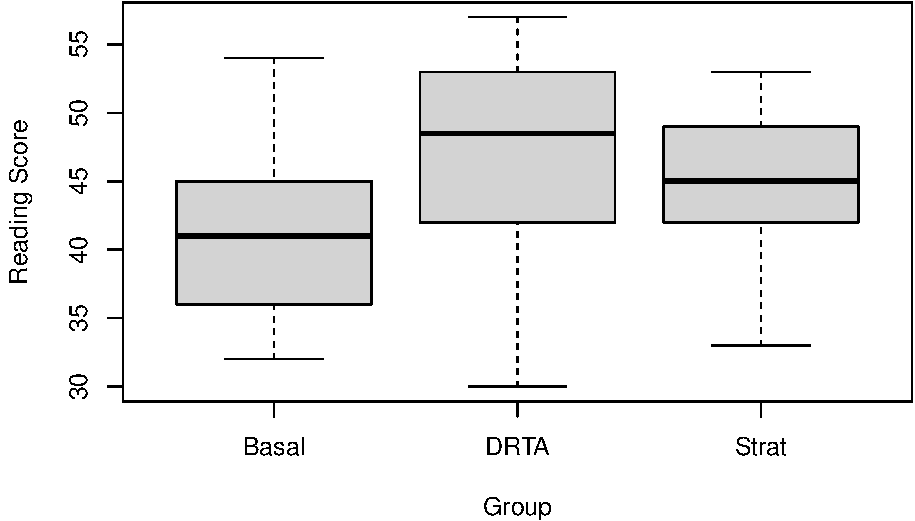
\includegraphics{emmeansNotes_files/figure-latex/unnamed-chunk-3-1.pdf}

The means and boxplots suggest that there may be systematic differences
in levels among the groups. The one-way ANOVA model can determine if the
difference is significative

\begin{Shaded}
\begin{Highlighting}[]
\KeywordTok{S}\NormalTok{(baum.mod}\FloatTok{.1}\NormalTok{ <-}\StringTok{ }\KeywordTok{lm}\NormalTok{(post.test}\FloatTok{.3} \OperatorTok{~}\StringTok{ }\NormalTok{group, }\DataTypeTok{data=}\NormalTok{Baumann))}
\end{Highlighting}
\end{Shaded}

\begin{verbatim}
Call: lm(formula = post.test.3 ~ group, data = Baumann)

Coefficients:
            Estimate Std. Error t value Pr(>|t|)    
(Intercept)   41.045      1.346  30.490  < 2e-16 ***
groupDRTA      5.682      1.904   2.985  0.00404 ** 
groupStrat     3.227      1.904   1.695  0.09498 .  
---
Signif. codes:  0 '***' 0.001 '**' 0.01 '*' 0.05 '.' 0.1 ' ' 1

Residual standard deviation: 6.314 on 63 degrees of freedom
Multiple R-squared: 0.1245
F-statistic: 4.481 on 2 and 63 DF,  p-value: 0.01515 
   AIC    BIC 
435.48 444.24 
\end{verbatim}

The pairwise comparisons of the means for the three groups can be
obtained using the \texttt{emmeans} function. emmeans comes form
``estimated marginal means'', the \emph{emmeans} package enables users
to easily obtain least-squares means for many linear, generalized
linear, and mixed models as well as compute contrasts or linear
functions of least-squares means, and comparisons of slopes.

\begin{Shaded}
\begin{Highlighting}[]
\NormalTok{(emms.est1.baum.mod}\FloatTok{.1}\NormalTok{ <-}\StringTok{ }\KeywordTok{emmeans}\NormalTok{(baum.mod}\FloatTok{.1}\NormalTok{, pairwise }\OperatorTok{~}\StringTok{ }\NormalTok{group))}
\end{Highlighting}
\end{Shaded}

\begin{verbatim}
$emmeans
 group emmean   SE df lower.CL upper.CL
 Basal   41.0 1.35 63     38.4     43.7
 DRTA    46.7 1.35 63     44.0     49.4
 Strat   44.3 1.35 63     41.6     47.0

Confidence level used: 0.95 

$contrasts
 contrast      estimate  SE df t.ratio p.value
 Basal - DRTA     -5.68 1.9 63 -2.985  0.0111 
 Basal - Strat    -3.23 1.9 63 -1.695  0.2150 
 DRTA - Strat      2.45 1.9 63  1.289  0.4064 

P value adjustment: tukey method for comparing a family of 3 estimates 
\end{verbatim}

\begin{Shaded}
\begin{Highlighting}[]
\NormalTok{(emms.est2.baum.mod}\FloatTok{.1}\NormalTok{ <-}\StringTok{ }\KeywordTok{emmeans}\NormalTok{(baum.mod}\FloatTok{.1}\NormalTok{, trt.vs.ctrl }\OperatorTok{~}\StringTok{ }\NormalTok{group))}
\end{Highlighting}
\end{Shaded}

\begin{verbatim}
$emmeans
 group emmean   SE df lower.CL upper.CL
 Basal   41.0 1.35 63     38.4     43.7
 DRTA    46.7 1.35 63     44.0     49.4
 Strat   44.3 1.35 63     41.6     47.0

Confidence level used: 0.95 

$contrasts
 contrast      estimate  SE df t.ratio p.value
 DRTA - Basal      5.68 1.9 63 2.985   0.0079 
 Strat - Basal     3.23 1.9 63 1.695   0.1712 

P value adjustment: dunnettx method for 2 tests 
\end{verbatim}

\begin{Shaded}
\begin{Highlighting}[]
\KeywordTok{plot}\NormalTok{(emms.est1.baum.mod}\FloatTok{.1}\NormalTok{)}
\end{Highlighting}
\end{Shaded}

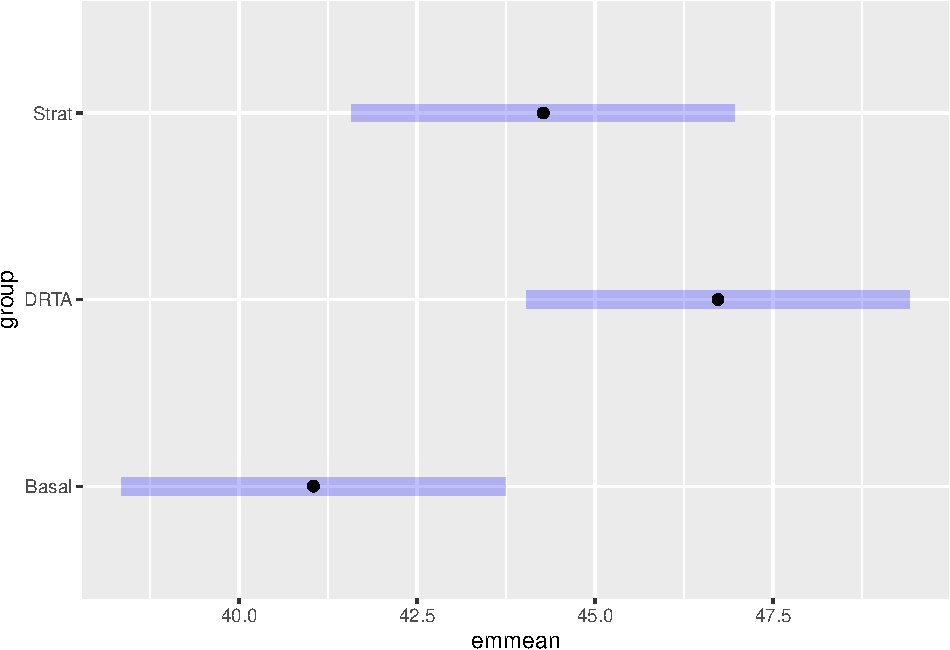
\includegraphics{emmeansNotes_files/figure-latex/unnamed-chunk-5-1.pdf}

\begin{Shaded}
\begin{Highlighting}[]
\KeywordTok{plot}\NormalTok{(emms.est2.baum.mod}\FloatTok{.1}\NormalTok{)}
\end{Highlighting}
\end{Shaded}

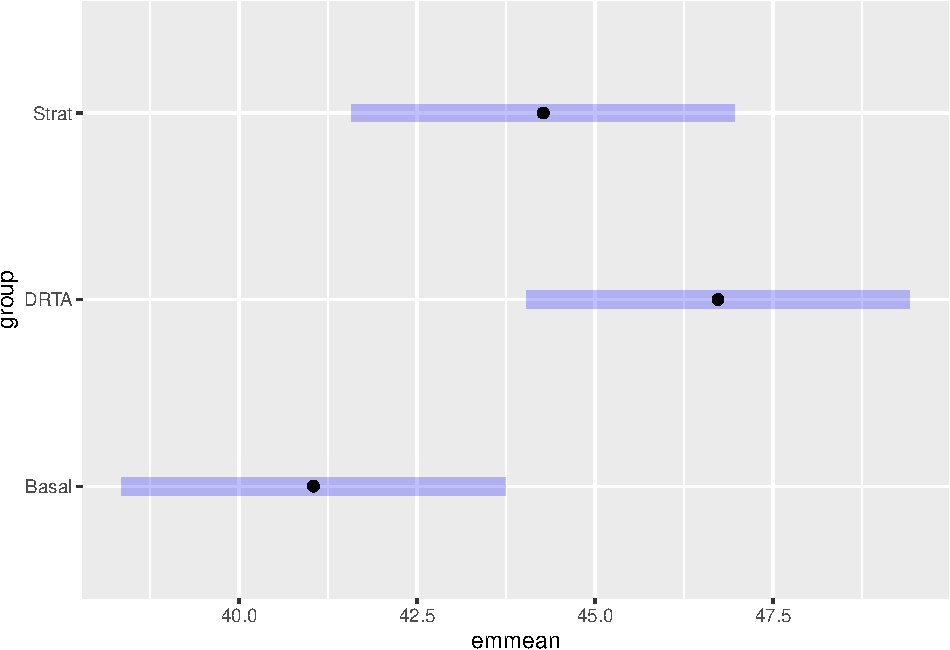
\includegraphics{emmeansNotes_files/figure-latex/unnamed-chunk-5-2.pdf}

\end{document}
